\chapter{Background and Related Work} \label{chap:background}
Providing a complete history of map and globe making (cartography) is much beyond both the scope and ability of this thesis.
Instead, this chapter aims to provide the necessary background to illuminate how these disciplines influenced the development of Digital Earth systems.
We go on to discuss the different approaches for a Digital Earth, starting with traditional GIS, and then techniques used for globe-based systems and analysis.
We also provide background and related work on discrete global grids and grid systems, looking at different methods for constructing these data structures.


\section{Traditional Maps and Globes} \label{chap:2:maps}
Cartography, the study and practice of making maps, is a mature and diverse discipline.
While there is no agreement on the earliest known map, there exist samples dating to the 4th millennium BCE and surviving world maps from 9th century BCE Babylonia.
Some may think of maps primarily as a navigation tool, but the uses extend much further.
Maps allow geospatial data (data with an associated geographic component) to be encoded, processed, and visualized in a scale reference.
Therefore, any field or discipline using such data often also uses maps of said data.


In the 3rd century BCE, the ancient Greeks established that the Earth is spherical; with this came the first globes of Earth.
Globes serve a similar purpose as maps; however, the use of a spherical reference as opposed to a planar one provides a more accurate representation of the Earth and helps prevent certain misinterpretations.
Despite this, maps were---and continue to be---the primary medium for representing the Earth and geospatial data~\cite{hruby20182000}.
Compared to maps, globes are more expensive to manufacture and more difficult to store, transport, and make measurements on.
Maps can also represent the entire Earth in one view and easily accommodate any scale.


\subsection{Map Projections} \label{chap:2:projection}
The benefits of a flat map over a globe do not come without their disadvantages.
Producing a map requires flattening the spherical Earth to a flat plane---an operation known as map projection (or simply projection)---which introduces inevitable distortions and the discontinuity of map edges.
Globes have no edges and significantly reduced distortion, and therefore provide a more accurate representation of the Earth than is possible with any map.
Despite these fundamental challenges, the many benefits of maps have motivated the use and study of these operations~\cite{snyder1987map, snyder1997flattening}.


Distortions in a map projection (or more generally in any mapping) are measured by their effect on angles, areas, and distances.
While eliminating all distortion is impossible, specialized projection methods exist that remove certain types of distortion.
Commonly used conformal (\cref{fig:mercator}) and area-preserving (\cref{fig:gall-peters}) projections preserve angles and areas, respectively.
Preserving distance also removes all other distortion, and since the sphere in non-developable, isometric projections between the sphere and the plane are impossible.
However, projections that preserve only certain distances, such as all those to a certain point, are achievable (\cref{fig:azi-equidist}).
Alternatively, some methods aim for a balanced tradeoff between the different types of distortion, as opposed to eliminating a specific type (\cref{fig:robinson}).


\begin{figure*}[htp!]
	\centering
	\begin{subfigure}[]{0.5\textwidth}
		\centering
		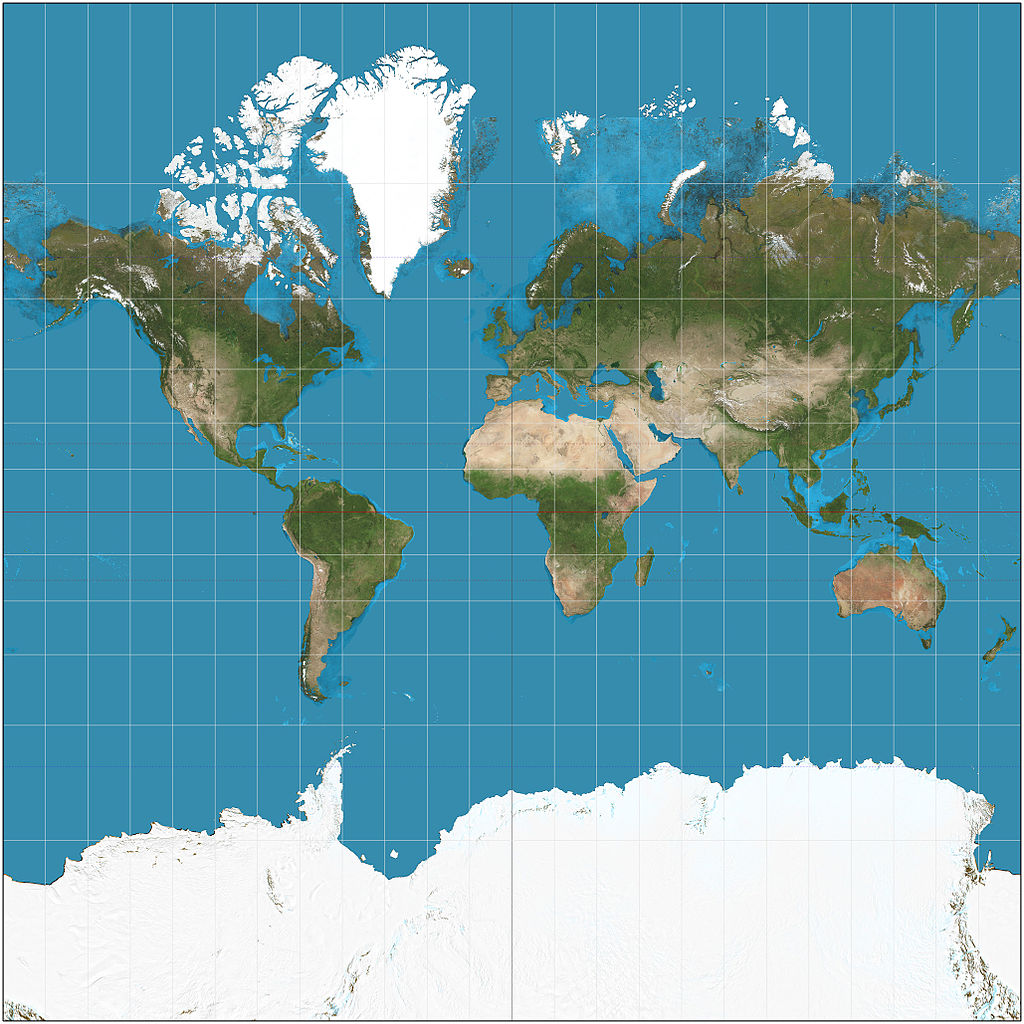
\includegraphics[width=0.95\textwidth]{mercator.jpg}
		\caption{}
		\label{fig:mercator}
	\end{subfigure}%
	%
	\begin{subfigure}[]{0.5\textwidth}
		\centering
		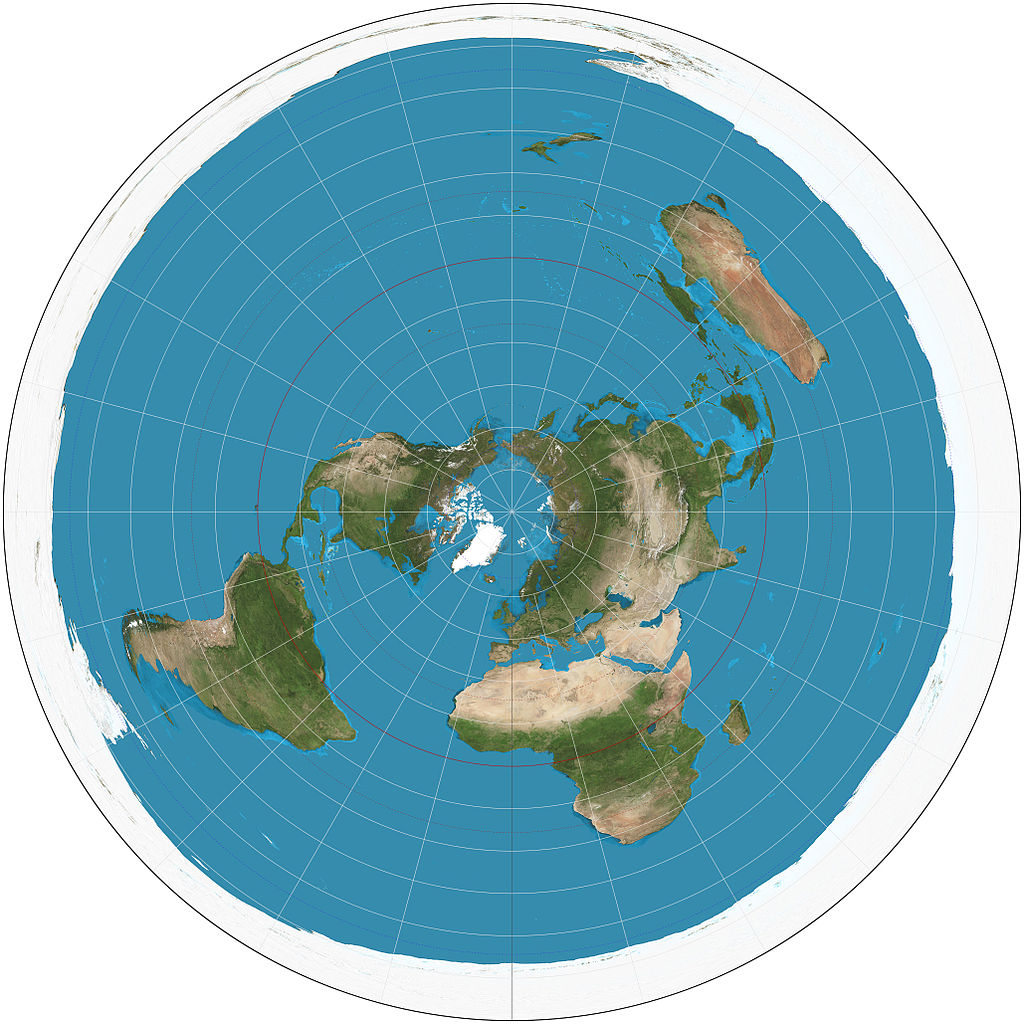
\includegraphics[width=0.95\textwidth]{azi-equidist.jpg}
		\caption{}
		\label{fig:azi-equidist}
	\end{subfigure}%
	
	\begin{subfigure}[]{0.5\textwidth}
		\centering
		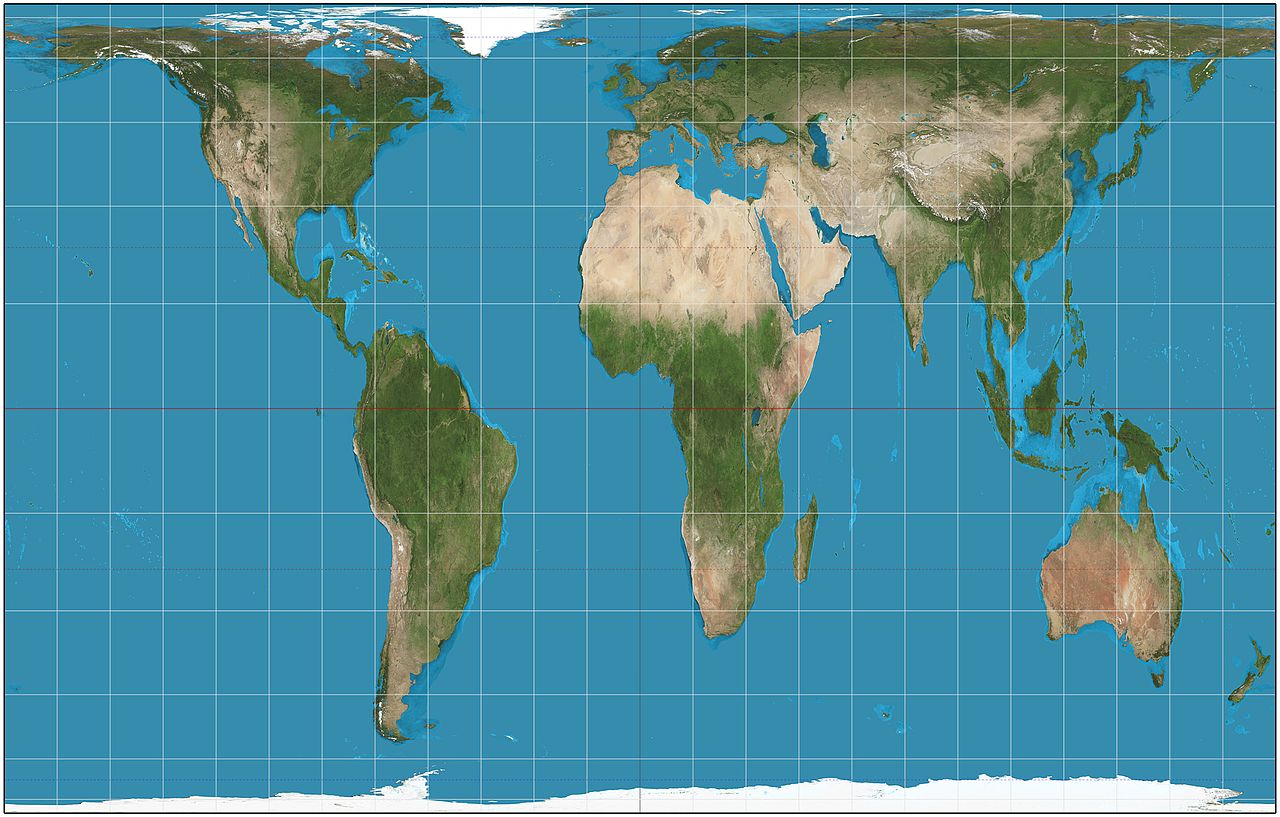
\includegraphics[width=0.95\textwidth]{gall-peters.jpg}
		\caption{}
		\label{fig:gall-peters}
	\end{subfigure}%
	%
	\begin{subfigure}[]{0.5\textwidth}
		\centering
		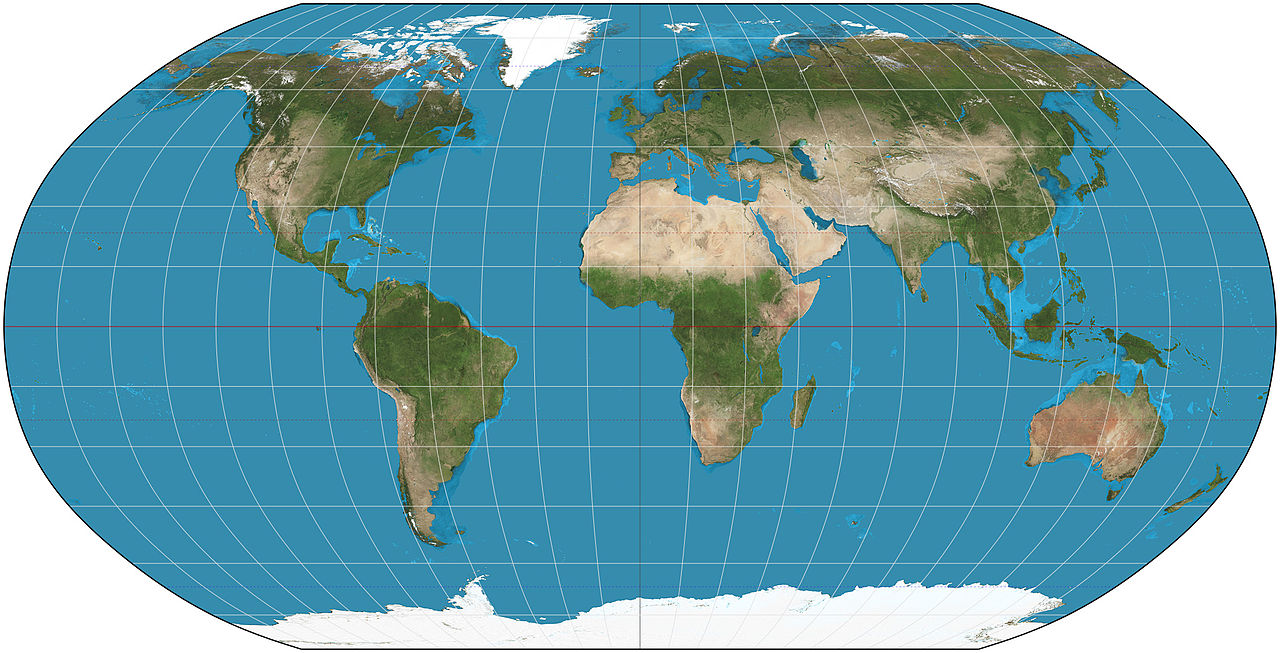
\includegraphics[width=0.95\textwidth]{robinson.jpg}
		\caption{}
		\label{fig:robinson}
	\end{subfigure}
	
	\caption[Four popular map projections]{
		Four common map projections and special properties they possess: (a) Mercator~\cite{mercator}, conformal; (b) azimuthal equidistant~\cite{azi-equidist}, equidistant to centre point; (c) Gall-Peters~\cite{gall-peters}, equal area; and (d) Robinson~\cite{robinson}, compromise (no measures preserved).
		Images courtesy of Daniel R. Strebe -- CC BY-SA 3.0
	}
	\label{fig:projections}
\end{figure*}


Since distortion cannot be completely removed, measurements and analyses done on flat maps can produce errors.
Straight lines may not map to the actual shortest path, area distortions may misrepresent the density of phenomena, and locations may appear much closer together or farther apart than they genuinely are.
The amount and type of error depend on the projection used and the type of analysis performed, with certain maps better suited for certain operations.
For example, the Mercator projection maps straight lines to rhumb lines making it a popular choice for navigation; however, the severely distorted area makes this projection a poor choice for representing the frequency of phenomena in different regions.
Therefore, it is essential to use an appropriate map projection for each intended use case, with no one projection being ideal in all circumstances.


\begin{figure}[ht!]
	\centering
	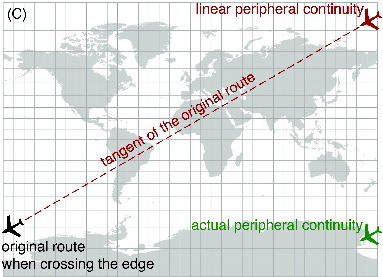
\includegraphics[width=0.55\textwidth]{edge-continuity.jpg}
	\caption[Actual vs. linear peripheral continuity on a map]{
		A demonstration of the actual and linear peripheral continuity of an object crossing the edge of a map.
		Image taken from~\cite{hennerdal2015beyond} with permission
	}
	\label{fig:edge-continuity}
\end{figure}


Another significant challenge with flat maps is the edges (or boundaries) introduced.
Such edges can have a significant impact on a person's understanding of a map when phenomena cross these boundaries.
A study by Hennerdal asked participants to predict the location and direction of an airplane crossing the boundary of different map projections~\cite{hennerdal2015beyond}.
The study found that participants would often incorrectly place the airplane at the point of \textit{linear} peripheral continuity (the intersection of the straight line tangent to the initial aircraft location and the opposite map edge) as opposed to the correct location (\cref{fig:edge-continuity}).
The occurrence of this mistake was most prominent with children; however, the effect was still present with adult participants. Another study by Hruby et al. measured how such edges impact the estimation of distance~\cite{hruby2016journey}.
Two groups of participants, given either a Eurocentric or Americentirc map to memorize locations, were asked to estimate the distances between various Asian and American cities.
While both groups overestimated distances on average, the group with the Eurocentric map (where the shortest distances crossed the map boundary), had larger estimation errors than the other group.
These studies further show that the projection used for a map must be chosen and centred carefully to ensure readers correctly understand how the map relates to the actual Earth.


\subsubsection{Polyhedral Projections} \label{chap:2:polyProj}
At the cost of introducing additional map edges, cutting a map can reduce the amount of distortion introduced by projection~\cite{soliman2018optimal}.
Such cuts are analogous to projecting the sphere to an underlying polyhedron, the net of which produces the final flat map.
\Cref{fig:poly-projection} shows one example of such a projection, the Dymaxion map.
Aside from reducing distortion, these polyhedron-based maps can serve as a pseudo-globe by folding the 2D net into the corresponding 3D polyhedron.


\begin{figure}[ht!]
	\centering
	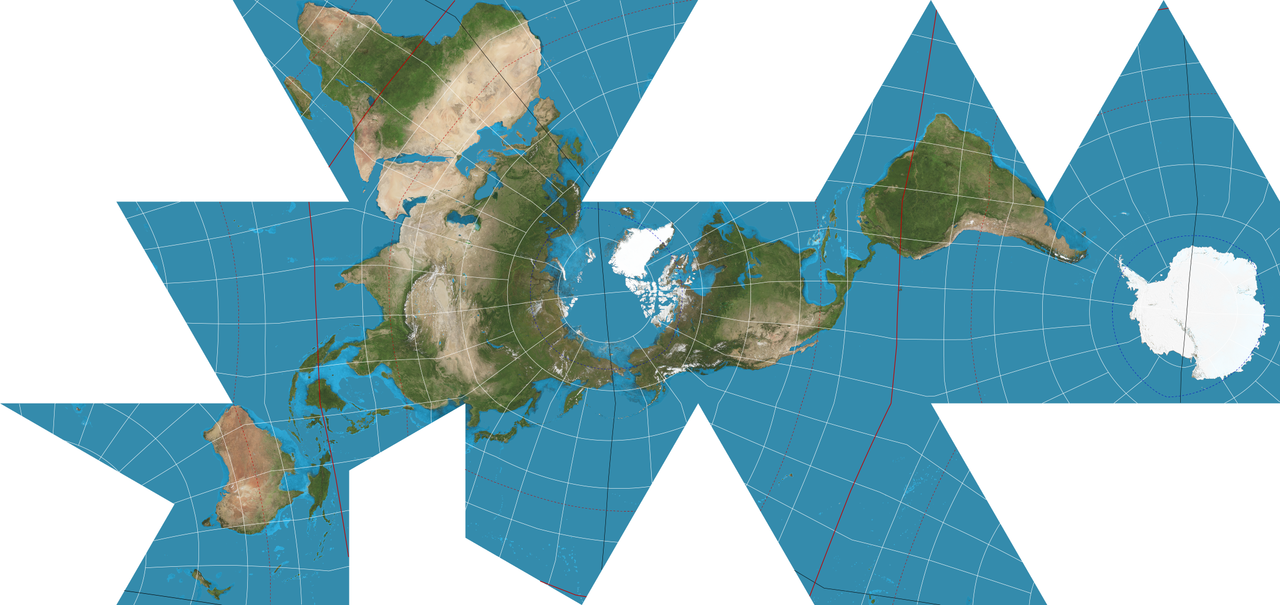
\includegraphics[width=\textwidth]{dymaxion.png}
	\caption[The Dymaxion (or Fuller) map projection]{
		The Dymaxion, also known as Fuller, map projection: one of the first examples of a polyhedron-based map projection.
		Image courtesy of Justin Haruaki Kunimune~\cite{dymaxion} -- CC BY-SA 4.0
	}
	\label{fig:poly-projection}
\end{figure}


Several works have developed area-preserving projections for different polyhedra.
Snyder modified the Lambert Azimuthal Equal-Area projection for use with all the platonic solids and the truncated icosahedron~\cite{snyder1992equal}; however, the inverse of this projection has no closed-form and requires an iterative solution.
Work has been done to improve the efficiency of this process~\cite{harrison2011optimization}.
Ro{\c{s}}ca and Plonka developed a closed-form projection and inverse for the cube~\cite{rocsca2011uniform} and octahedron~\cite{rocsca2012area}.
Subsequently, Holho{\c{s}} and Ro{\c{s}}ca proposed an alterative projection for the octahedron derived off of different principles~\cite{holhocs2014octahedral}.
van Leeuwen and Strebe also developed a class of projections for the platonic solids~\cite{van2006slice}, one of which was later adapted to the disdyakis triacontahedron~\cite{hall2020disdyakis}.


\section{Digital Earth Systems} \label{chap:2:DE}
With the advent of computing systems came the move of maps from the physical domain to the digital one.
Initially, this required scanning existing physical maps to digitize the data they contained.
As the prevalence of computers increased, more geospatial data was stored natively in digital formats.
Nowadays, nearly all (if not all) geospatial data is collected and stored digitally.
Furthermore, advancements in remote sensing technologies, smart technologies, and the Internet of Things have led to explosive increases in the amount of geospatial data collected.
Modern computers can process vast amounts of data compared to what is possible manually; despite this, the volume and complexity of geospatial data available and being collected surpasses even this capacity~\cite{lee2015geospatial}.


To make full use of the geospatial data gathered by society, former US vice president Al Gore proposed the idea of a Digital Earth~\cite{gore1998}.
This Digital Earth---a 3D virtual globe---would serve as a common reference for the vast majority of geospatial data to be freely accessible by the public.
This vision has since been further refined to be not one, but several connected Digital Earths that individually better meet the needs of specific audiences~\cite{goodchild2012next}.
Currently, many different systems exist for creating a Digital Earth with significant variations in methodology, scope, and intended use(s).


\subsection{Geographic Information Systems} \label{chap:2:GIS}
Long before Al Gore's idea of a Digital Earth, traditional cartography techniques were being applied to systems for creating and managing digital maps.
These technologies became what is known today as GIS~\cite{foresman1998history}.
Just as with physical maps, in a GIS, different datasets are represented as individual layers in a shared coordinate system.
Different layers can then be integrated and analyzed through combinations of set operations (union, intersection, and difference), statistical analysis (e.g. mean and standard deviation), and other operations.
These integrations and analyses are also used to create visualizations of the underlying data.


Since their introduction, GIS has proven to be a powerful framework for managing geospatial data.
This power, however, is a double-edged sword; proper use of a GIS requires a significant amount of knowledge and expertise~\cite{antenucci1991geographic}.
To be used with a GIS, geospatial data must first be cleaned, remapped, processed, integrated, and distributed.
All of these operations require familiarity with both the system used and the underlying cartographic principles.
Furthermore, due to the frequent use of a planar coordinate system, distortion from projection can introduce errors in analysis and visualization, just as with physical maps.
Which map projection to use for which use cases must be considered carefully, which also requires sufficient domain expertise.


\subsection{Globe-Based Digital Earth} \label{chap:2:globeDE}
A more recent approach to a Digital Earth---and one more in line with Al Gore's initial proposal---is a globe-based Digital Earth.
While physical globes have practical drawbacks compared to a physical map, in a digital setting, these drawbacks are reduced if not completely negated.
Modern computer graphics algorithms and hardware have made creating, storing, and displaying a virtual globe in real-time no more difficult than displaying the equivalent map.
Interactive systems allow zooming, panning, and rotating the globe to show any region of Earth at the desired scale.
Virtual globes still cannot display the entire Earth at once; however, novel interaction techniques such as multi-view focus plus context rendering can help alleviate this limitation~\cite{sherlock2017visualizations}.


Due to the reduced distortion with a globe, there has been a push toward globe-based Digital Earth systems as opposed to conventional map-based ones~\cite{goodchild2018reimagining}.
One approach for doing so is to still use a flat map as the underlying representation of the Earth but map back to a globe for visualization.
While this solves the issues of map edges and provides a more accurate reference for visual analysis, it does not address the distortion present for any analysis using the flat map and the corresponding errors introduced.
The alternative is to do analysis directly in spherical---or even more accurately, ellipsoidal---space.
While ellipsoidal analysis is often prohibitively complicated and expensive due to the mathematical challenges of elliptic integrals~\cite{byrd2013handbook}, techniques for spherical analysis are well understood~\cite{raskin1994spatial}.
While spherical analyses are still significantly more involved than the planar equivalents, modern computational capabilities are making them more feasible. 
In addition to standard methods, there are several recent works on techniques for more complex spherical analysis and operations.
Some examples include better representations for rational points on the sphere~\cite{bahrdt2017rational}, multiresolution representations of B-spline~\cite{alderson2016multiresolution} and NURBS curves~\cite{alderson2019multiscale}, and methods for offsetting both vector and raster curves~\cite{alderson2018offsetting}.
For these reasons, direct spherical analysis on a globe-based Digital Earth is becoming a compelling alternative to traditional GIS. For a detailed analysis of different Digital Earth systems, refer to~\cite{mahdavi2015survey} and~\cite{alderson2020digital}.


\subsection{Volumetric Digital Earth} \label{chap:2:VDE}
While most Digital Earth systems focus primarily on the Earth's surface, several properties and activities exist above and below the surface that affect the planet.
These include, but are not limited to, tectonic plate movement, ocean currents, global weather, air quality and pollutants, and reservoir locations.
Correspondingly, there are datasets available about the events in these regions, which some Digital Earths work to process and integrate.
We call such a system a \textit{volumetric} Digital Earth, as it is concerned with the Earth as a volume as opposed to just a surface.


One notable example of a volumetric Digital Earth is the use of atmosphere and weather observations for global numerical weather predictions and reanalysis~\cite{ncepncar, era5}.
These datasets are freely publically available; however, they require domain expertise and tools in order to process and understand.
Instead, third parties such as Windy\footnote{\url{https://www.windy.com/}} and Ventusky\footnote{\url{https://www.ventusky.com/}} have produced visualizations of these datasets to make them more readily available to the public.


Thus far, volumetric Digital Earths have mostly been limited to scientific applications as opposed to platforms intended for use by the public.
Chapter 3 provides more examples of volumetric Digital Earths through the lens of the grid systems they employ, which include lithosphere visualizations, aircraft collision detection, volumetric atmosphere rendering, and encoding LIDAR point cloud data.


\section{Discrete Global Grids} \label{chap:2:DGG}
Space partitioning data structures have long been used in computer graphics to aid various geometry querries~\cite{samet1990design}.
These data structures provide information about which objects are near others and prevent unnecessary queries and tests between distant geometries.
Common examples of this type of data structure include voxel grids, k-d trees, binary spatial partitioning (BSP) trees, and quad/octrees.
Space partitionings, particularly compact and uniform ones, are also useful for the sampling and aggregation of data. 


Similarly, space partitionings of the Earth for geospatial data are also useful.
However, due to the spherical nature of the Earth, different techniques are often used as opposed to the above methods designed for Euclidean spaces.
A Discrete Global Grid (DGG) partitions the surface of the Earth into a set of non-overlapping cells allowing geospatial data to be associated with the appropriate cell(s).
There exist several different approaches for creating a DGG, each with benefits and drawbacks.
Likewise, the specific uses of a DGG vary based on the Digital Earth system.
In some systems, a DGG only serves as a data structure for speeding up various spatial queries and analyses.
Other entities have used a DGG (more specifically, a DGGS---described in more detail below) as the foundation and framework for an entire Digital Earth system~\cite{peterson2011close}.
Regardless of their specific use(s), DGG's are an essential aspect of many Digital Earths and, as such, are well studied.


\subsection{Discrete Global Grid Systems} \label{chap:2:DGGS}
While DGG's are a helpful tool, they only represent the Earth at one spatial resolution.
If only working with one dataset, this is adequate; however, geospatial data comes in a wide range of resolutions, so multiple resolutions of DGG's may be needed when working with multiple datasets.
This shortcoming is addressed with a hierarchy of DGG's at increasingly fine resolutions, also known as a Discrete Global Grid System (DGGS)~\cite{sahr1998discrete, sahr2003geodesic}.
Such a hierarchy allows geospatial data at any spatial resolution to be appropriately integrated at its native resolution and used with any other dataset.


\subsubsection{Refinement} \label{chap:2:refinement}
The most common approach for creating a DGGS is by defining an initial discretization and cell refinement method~\cite{mahdavi2015survey}.
The initial discretization is a DGG that serves as the most coarse level of the hierarchy. The cell refinement method defines a process for creating the next level of the hierarchy from the previous.
If done systematically and consistently, refinement can be applied successively to create arbitrarily fine discretizations of the Earth.


Different refinement schemes are classified by their input cell shape(s), which are given by the initial discretization; output cell shape(s), which are usually the same as the input; and their refinement factor, which is simply the ratio between the number of coarse and fine cells.
For example, triangle 1-to-4 (1:4) refinement produces four fine triangle cells for each triangle in the set of coarse cells.
The refinement factor determines how quickly the resolution of the grid increases with each application of the refinement method, with lower ones usually preferred in order to represent the Earth at a higher number of resolutions.


Refinement should also maintain the relative shape of cells between different resolutions of the DGGS.
For example, refining square cells should produce (roughly) square cells, and not increasingly skinny rectangles.
This property ensures that refinement maintains the compactness and aspect ratio of cells between different resolutions of the grid system.
Two other noteworthy properties of refinement are congruency and alignment.
With congruent refinement, each coarse cell is composed of a union of fine cells.
Aligned refinement requires that each coarse cell shares a certain point with a fine cell, usually either a vertex or centroid (for vertex-aligned and centre-aligned refinement, respectively).
Congruency and alignment are not required properties of refinement but are desirable in certain situations.
Furthermore, based on other requirements of the refinement method, these properties may be unattainable. For example, congruent refinement is impossible for hexagon cells.
A more thorough investigation of these properties is available in~\cite{mahdavi2015survey}.


As an aside, in the literature, the term subdivision is used interchangeably with refinement.
While these terms are equivalent in the context of a DGGS, in the computer graphics literature, subdivision typically refers to subdivision curves and surfaces~\cite{bohm1983sudividing, catmull1978recursively, loop1987smooth}: processes that involve vertex repositioning.
For consistency and to avoid confusion, this thesis exclusively uses the term refinement to refer to the process of creating a set of fine cells from a set of coarse ones, even if vertex repositioning is a part of this operation.


\subsection{Spherical Grids} \label{chap:2:spherical}
With the Earth commonly approximated as a sphere, many DGG's and DGGS's are defined directly in this space.
One of the most straightforward approaches for doing so is with a regular discretization based on latitude and longitude coordinates, or a latitude-longitude grid (LLG), shown in \cref{fig:llg}.
Similar to a regular grid in Euclidean space defined by equal steps in Cartesian coordinates, an LLG divides the sphere into equal steps of latitude and longitude.
Unlike Cartesian coordinates, however, spherical coordinates have singularities at both poles causing quadrilateral LLG cells to degenerate into triangles.
These singularities reduce the size and compactness of cells near the poles, resulting in significant area differences between cells in the grid; they also produce a high valence vertex at each pole.
Thus, an LLG is neither a compact nor uniform DGG.


\begin{figure}[ht!]
	\centering
	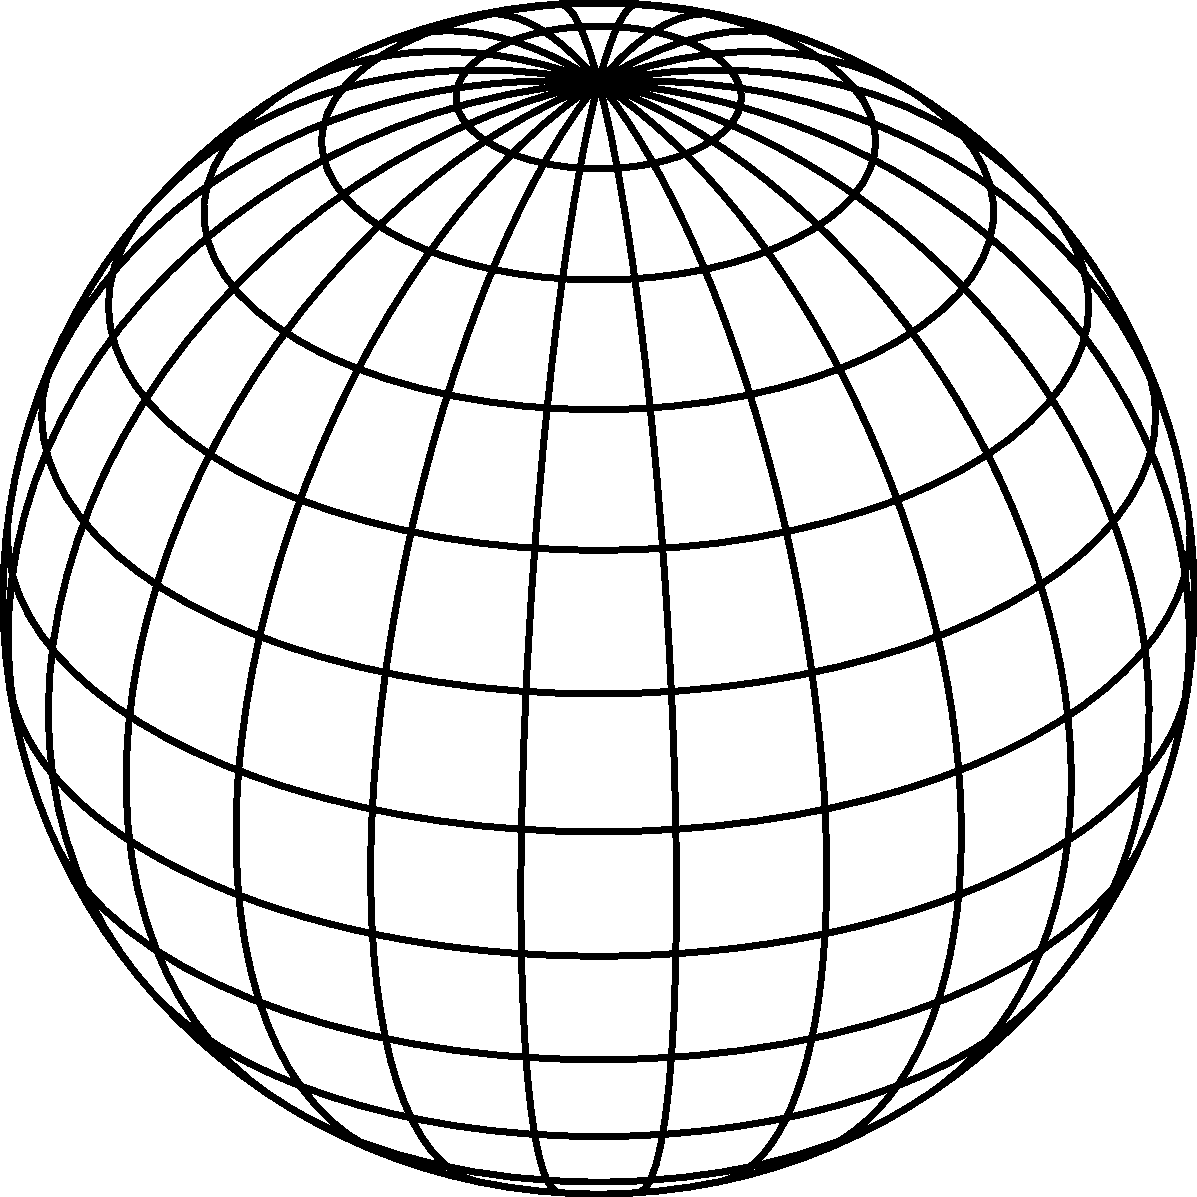
\includegraphics[width=0.4\textwidth]{llg.pdf}
	\caption[A latitude-longitude grid]{
		\textbf{Placeholder and temporary caption} A latitude-longitude grid (LLG) with 24 longitudinal division and 12 latitudinal divisions.
		Note how cells become increasingly narrow toward poles, resulting in reduced size and compactness as compared to cells more near the equator
	}
	\label{fig:llg}
\end{figure}


As (absolute) latitude increases, the same angular longitude corresponds to decreasing arc lengths on the sphere.
Because of this, one strategy to lessen the drawbacks of an LLG is to increase the longitude step size as (absolute) latitude increases.
Modifying an LLG in this way results in more uniform sized and compact grid cells at the cost of introducing irregular and degenerate connectivity to the grid.
We explore this tradeoff more in \cref{chap:3:semiregDegen}.
Using this strategy, Leopardi provides a formulation for creating an equal area and compact partitioning of the sphere into any number of regions~\cite{leopardi2006partition}.
Similarly, the Degenerate Quadtree Grid (DQG) proposed by Sun et al. makes use of a modified quadtree refinement to create this type of grid~\cite{sun2008global}.
The use of a refinement method---along with the provided encoding, decoding, and indexing algorithms---allows the DQG to operate as a full DGGS as opposed to just a single resolution DGG.


Another approach that solves some of the issues with a simple LLG is the Yin-Yang grid proposed by Kageyama and Sato~\cite{kageyama2004yin-yang}.
This grid is composed of two congruent component grids---the Yin and Yang grids---which are LLG's 270\textdegree \ in longitude and 90\textdegree \ in latitude centred at the equator.
These component grids are then rotated and placed atop each other to cover the sphere fully.
As the component grids have a limited latitude, they do not have the same compactness and area issues seen in an LLG.
However, cells near the boundaries of the component grids overlap in the composite grid creating either ambiguity or redundancy when associating geospatial data with cells and complicating grid connectivity in these regions.


A different method for defining a grid in spherical space is to forgo latitude and longitude coordinates altogether, and instead use arbitrary curves to define the edges of the grid.
One such method by Song et al. uses small circle arcs to perform an equal area triangle refinement directly on the sphere~\cite{song2002developing}.
While the resulting cells are equal area and have good compactness properties, calculating the correct small circle arcs to use during refinement has no known analytical solution and therefore requires an iterative approximation.
Furthermore, these types of grids have more expensive operations, often requiring a hierarchical algorithm (linear time on the level of refinement) as opposed to a direct (constant time) one.


\subsection{Polyhedral Grids} \label{chap:2:polyhedral}
As opposed to defining the grid directly in spherical space, a more recent and increasingly popular approach is to use a polyhedron as an initial approximation of the sphere.
The most common choices for these polyhedra are the Platonic solids, as they are perfectly regular; however, other choices are also possible.
Mapping back and forth between the Earth and polyhedron is accomplished using a polyhedral map projection and its inverse, respectively.
From this, a planar refinement of the polyhedron faces creates the cell hierarchy for a DGGS.
This style of grid avoids degeneracies in the grid at the poles, providing a more uniform discretization of the entire Earth compared to grids based on latitude and longitude coordinates.
Furthermore, the use of an area-preserving projection in conjunction with an area-preserving refinement of the polyhedron allows for an equal area grid without a significant reduction in cell compactness.


\begin{figure}[ht!]
	\centering
	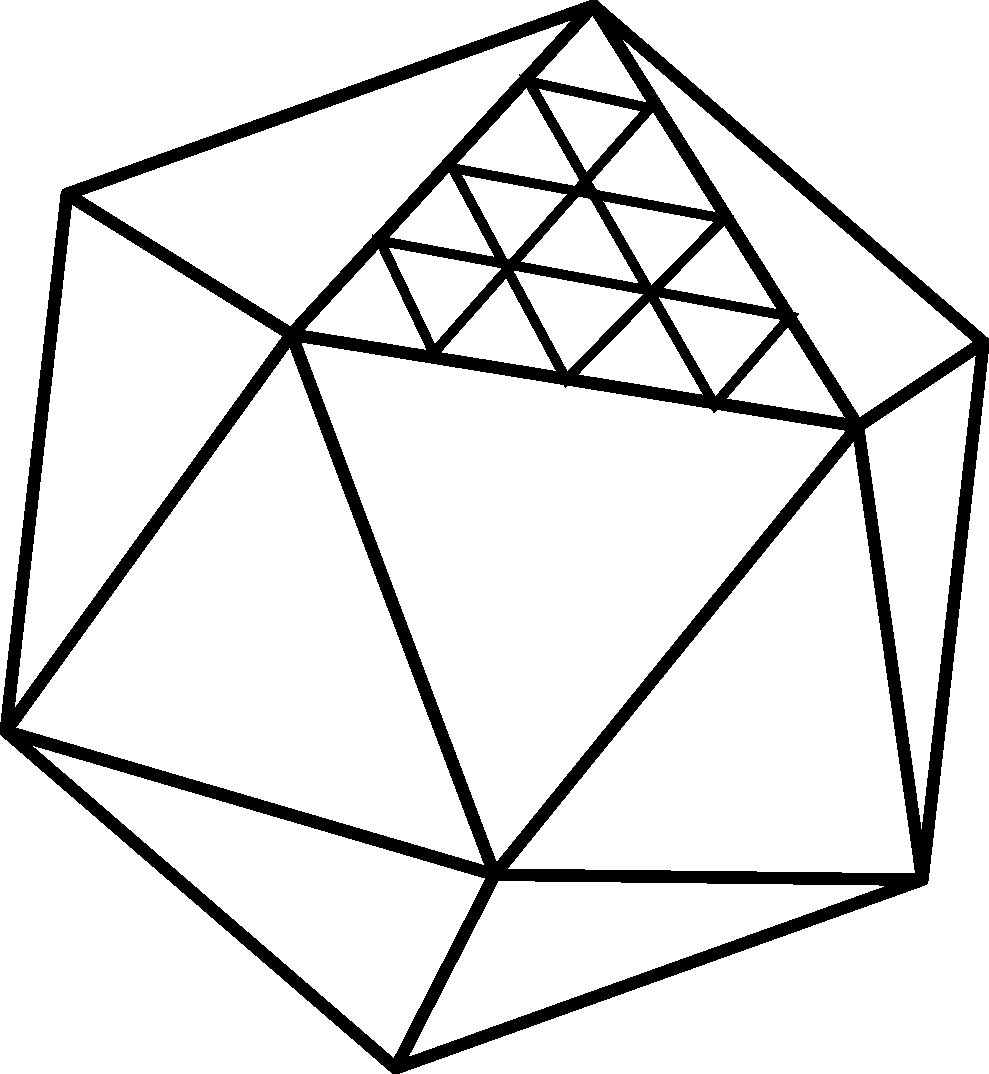
\includegraphics[width=0.30\textwidth]{polyhedron-grid.pdf}
	\caption[An icosahedron-based grid]{
		\textbf{Placeholder and temporary caption} A simple triangular grid based on a regular icosahedron.
		Probably also show projection between polyhedron domain and spherical domain
	}
	\label{fig:poly-grid}
\end{figure}


One of the earliest polyhedron-based DGGS's is the Sphere Quadtree, proposed by Fekete in 1990~\cite{fekete1990sphere}.
This system uses a regular icosahedron as the initial discretization, along with standard 1:4 triangle refinement.
The authors use a normalization projection to map between the sphere and icosahedron: a line originating at the centre of the sphere intersects the sphere and icosahedron once, and these two intersections define the projection and its inverse.
Dutton later adopted a similar method to the regular octahedron~\cite{dutton1996encoding}.
While these two approaches are straightforward, they served as the groundwork for more sophisticated polyhedron-based DGGS's.
Some more recent examples include HEALPix~\cite{gorski2005healpix}, ISEA3H~\cite{sahr2003geodesic}, SCENZ-Grid~\cite{scenz}, One-to-Two Digital Earth~\cite{mahdavi2013one}, and Disdyakis Triacontahedron DGGS~\cite{hall2020disdyakis}.
The Open Geospatial Consortium (OGS) has created a standard working group and an abstract specification for DGGS's~\cite{ogcDGGS, purss2016ogc}.
These efforts work to standardize the creation of DGGS's and outline the desired properties of the resulting systems.
We again refer to~\cite{mahdavi2015survey} and~\cite{alderson2020digital} for a more detailed analysis and comparison of different DGGS's.


\subsection{Grid Encoding and Decoding} \label{chap:2:coding}
For a DGG or DGGS to be useful as a tool for managing geospatial data, operations are needed that can associate said data with the appropriate set of cells.
This class of operations is known as grid encoding.
The most basic type of encoding is for points---finding the cell which contains a given point---however, operations for more complex geometry such as vector polylines and polygons is often also required~\cite{du2018duality}.
Likewise, the inverse process of mapping a set of cells in the grid domain to the corresponding regions of the Earth is also needed.
These operations are, correspondingly, known as grid decoding.
Grid encoding and decoding, as they apply to a polyhedron-based grid, are shown in \cref{fig:coding}.
In this thesis, we refer to grid encoding and decoding collectively as coding.


\begin{figure}[ht!]
	\centering
	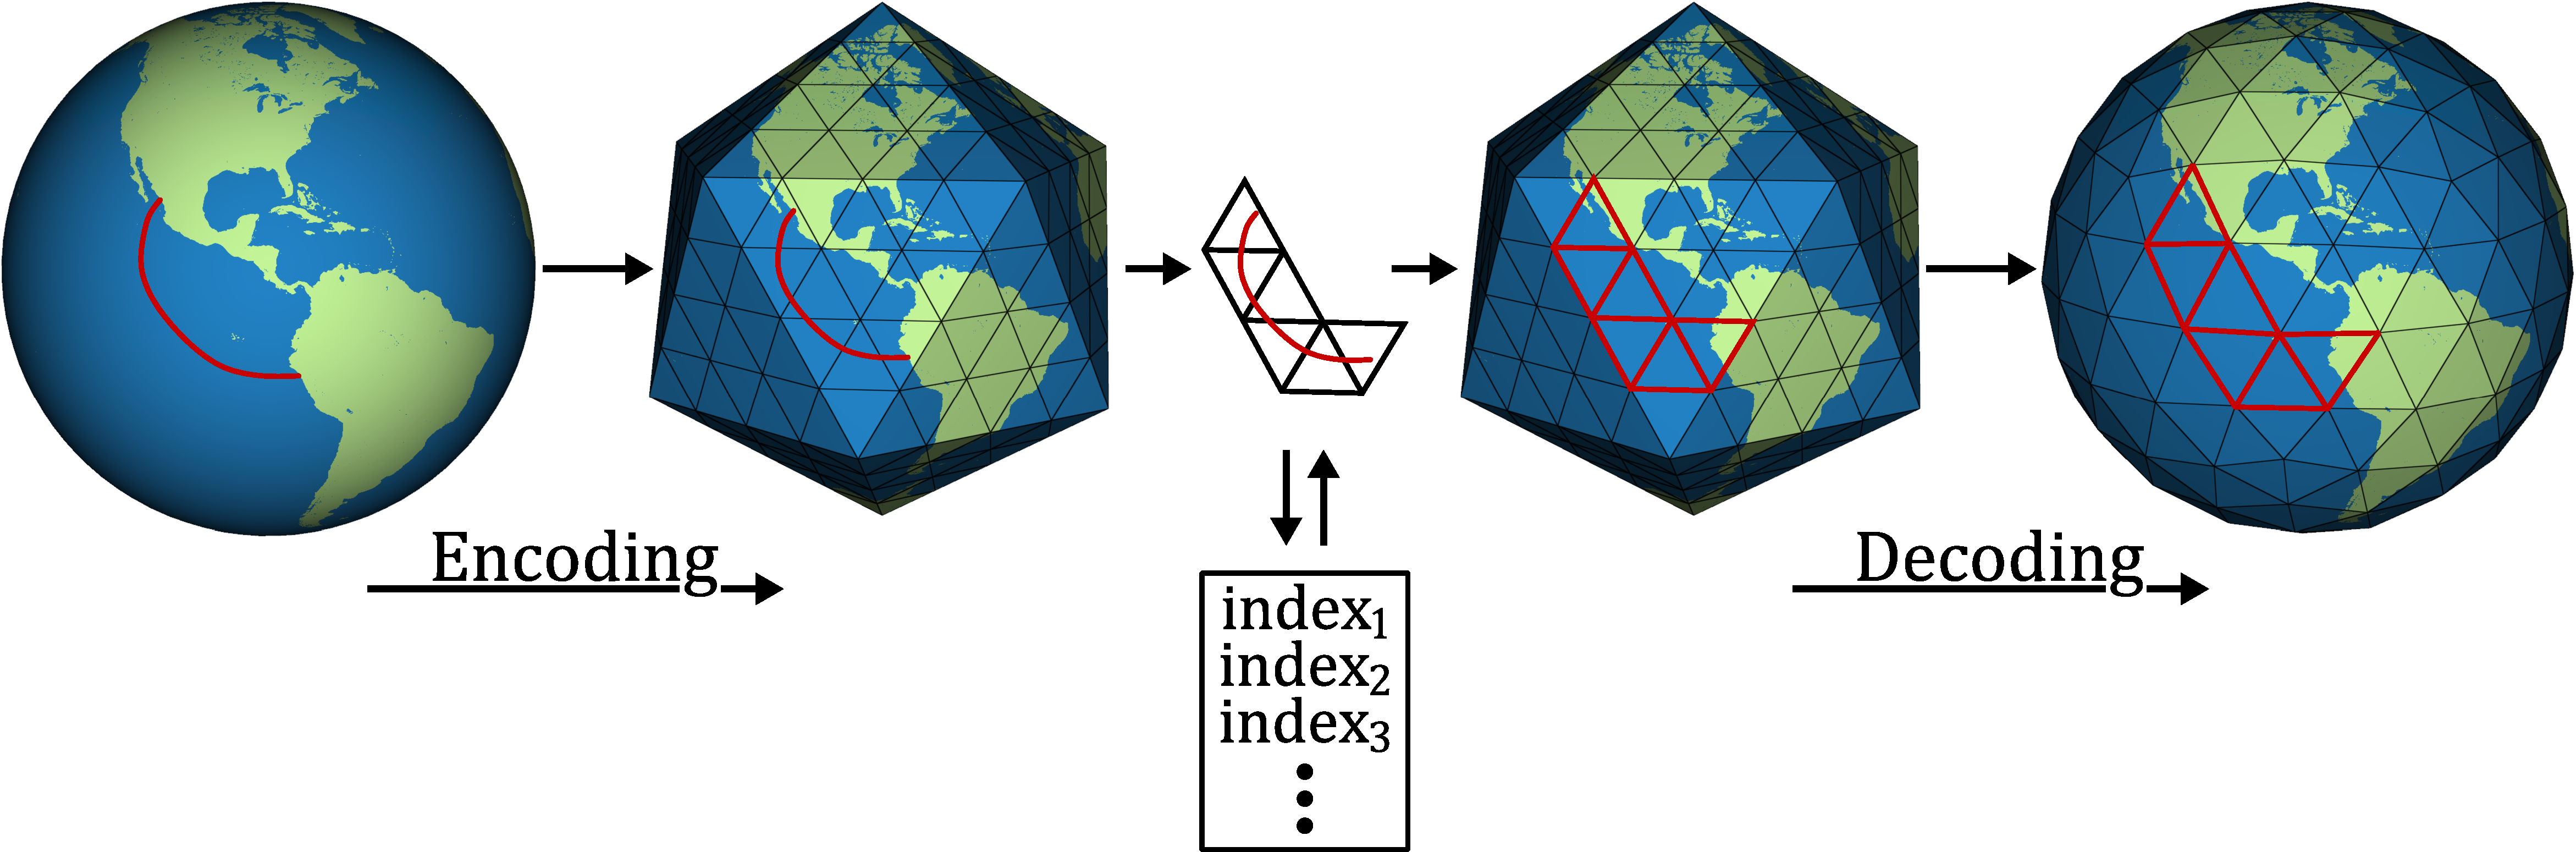
\includegraphics[width=\textwidth]{coding.pdf}
	\caption[Grid encoding and decoding with a polyhedral grid]{
		The process of encoding (left) and decoding (right) with a polyhedral grid.
		Encoding: features are projected from the Earth domain to the polyhedral domain of the grid; the set of planar cells associated with the feature are obtained---each of which has a unique index.
		Decoding: a set of cell indices corresponds to cell geometry on the polyhedral grid; cells in the polyhedral domain are inverse projected back to the Earth domain
	}
	\label{fig:coding}
\end{figure}


\subsubsection{Indexing Scheme} \label{chap:2:indexing}
Closely related to coding operations is the method used to assign a unique identifier to each cell in a DGG or DGGS.
Such an index is necessary in order to unambiguously distinguish between cells in the grid so that data can be associated with a set of cells via association with the corresponding index or indices.
Indices are also used to traverse through the grid with neighbour relationships and, in a DGGS, traverse the hierarchy with parent and child relationships.


In a given scheme, indices may have different representations depending on the context, with (injective) functions that convert between different representations.
As an example, for a regular quadrilateral grid, a natural choice for assigning unique identifiers to each cell is with a 2D coordinate-based index~\cite{mahdavi2015survey}.
This choice allows straightforward and constant-time algorithms for several operations: encoding of points represented in the same coordinate system, decoding of cells to obtain the minimum and maximum in each dimension, and retrieving the index of neighbouring cells in the grid.
However, standard row-major and column-major linearizations of these coordinates may not be ideal for storing data associated with said indices.
When performing grid operations, it is more likely to require additional data from a nearby region than from a distant region.
Therefore, nearby cells should ideally have similar indices to decrease the number of cache misses and disk seeks; row-major and column-major orderings do not have this property.
In our example then, a different representation of the indices---such as one derived from a space-filling curve---may be used when storing and retrieving data~\cite{morton1966computer}.


The exact method used to index cells depends heavily on the geometry of the grid itself.
For example, an indexing scheme designed for a regular quadrilateral grid is unlikely to be useful (or even applicable) to an irregular triangle grid.
Thus, grids with different cell shapes and connectivities require different indexing schemes designed specifically for the qualities of that grid.
Regular quadrilateral and triangular grids have well-understood techniques for indexing from the computer graphics literature.
Furthermore, Atlas of Connectivity Maps---proposed by Mahdavai-Amiri and Samavati---extend these techniques to semiregular grids like those of most polyhedral DGGS~\cite{mahdavi2014atlas}.
However, hexagon-based grids, which are an increasingly popular choice due to their desirable sampling properties resulting from the high compactness of hexagons, are more difficult to index.
Despite this, there are some works on developing efficient indexing for both 1:3~\cite{vince2006indexing} and 1:4~\cite{tong2013efficient} hexagon DGGS's, along with general methods for hierarchical hexagonal grids~\cite{mahdavi2015hexagonal}.
There has also been work done to categorize different DGGS indexing schemes to facilitate conversion and data transference between different systems~\cite{mahdavi2015categorization}.


\section{Summary} \label{chap:2:summary}
The world we live in is full of data, and maps of globes of the Earth have a long history in helping people understand and process that data.
With maps historically favoured over globes for practical reasons, digital representations have allowed for virtual globes that more accurately represent the Earth as compared to flat maps.
Computers have also increased the amount of geospatial data we can process, but---along with other technologies---have also led to an explosion in the amount of data available.
In handling this ever-increasing amount of data, DGG's and DGGS's have become an essential tool in addition to conventional GIS technologies.
While there exist many different techniques for creating these global grids, those based on approximating polyhedron have become the state-of-the-art choice.
The 3D DGGS, which we explore more in the next chapter, is the next step in this evolution for facilitating the efficient integration, analysis, and visualization of geospatial data for a volumetric Digital Earth.
